\documentclass[10pt,aspectratio=43]{beamer}
%\mode<presentation> {
%	%\usetheme{CambridgeUS}
%	\usecolortheme{dolphin}
%}
\usepackage{nju}			 %导入 nju 模板宏包
%\usepackage[UTF8]{ctex}      %导入 ctex 宏包,添加中文支持
%\usepackage{xeCJK}
\usepackage{amsmath,amsfonts,amssymb,bm}   %导入数学公式所需宏包
\usepackage{color}			 %字体颜色支持
\usepackage{graphicx,hyperref,url}
\usepackage{listings}
\usepackage{booktabs}
\usepackage{multirow}
\usepackage{float}
\usepackage[version=4]{mhchem}
\usepackage{animate}
\usepackage[isbn=false,doi=false,url=false,uniquename=init,style=chem-acs]{biblatex}
\addbibresource{icc_proj.bib}
\AtEveryCitekey{\clearfield{title}}
\AtEveryBibitem{\clearfield{title}}
\usepackage{textcomp}
\usepackage{multicol}
\usepackage{fontspec}
\setmainfont{Times New Roman}
\setsansfont{Arial}
\setmonofont{Courier New}

\usepackage{listings}
\definecolor{dkgreen}{rgb}{0,0.6,0}
\definecolor{gray}{rgb}{0.5,0.5,0.5}
\definecolor{mauve}{rgb}{0.58,0,0.82}
\lstset{ %
	language=Python,                % the language of the code
	basicstyle=\Consolas\footnotesize,           % the size of the fonts that are used for the code
	numbers=left,                   % where to put the line-numbers
	numberstyle=\tiny\color{gray},  % the style that is used for the line-numbers
	stepnumber=1,                   % the step between two line-numbers. If it's 1, each line 
	% will be numbered
	numbersep=5pt,                  % how far the line-numbers are from the code
	backgroundcolor=\color{white},      % choose the background color. You must add \usepackage{color}
	showspaces=false,               % show spaces adding particular underscores
	showstringspaces=false,         % underline spaces within strings
	showtabs=false,                 % show tabs within strings adding particular underscores
	frame=single,                   % adds a frame around the code
	rulecolor=\color{black},        % if not set, the frame-color may be changed on line-breaks within not-black text (e.g. commens (green here))
	tabsize=4,                      % sets default tabsize to 2 spaces
	captionpos=b,                   % sets the caption-position to bottom
	breaklines=true,                % sets automatic line breaking
	breakatwhitespace=false,        % sets if automatic breaks should only happen at whitespace
	title=\lstname,                   % show the filename of files included with \lstinputlisting;
	% also try caption instead of title
	keywordstyle=\color{blue},          % keyword style
	commentstyle=\color{dkgreen},       % comment style
	stringstyle=\color{mauve},         % string literal style
	escapeinside={\%*}{*)},            % if you want to add LaTeX within your code
	morekeywords={*,...}               % if you want to add more keywords to the set
}
\usepackage{multicol}
\usepackage{multirow}
\usepackage{siunitx}
\definecolor{codegray}{gray}{0.9}
\newfontfamily\Consolas{Consolas}
\newcommand{\code}[1]{\colorbox{codegray}{{\Consolas#1}}}
\newcommand{\hl}[1]{\colorbox{yellow}{#1}}
\lstnewenvironment{mcode}
{\lstset{backgroundcolor=\color{lightgray},
		xleftmargin=0.5cm,
		frame=tlbr,framesep=4pt,framerule=0pt,
		%language=python,
		keepspaces=false,
		numbers=none
}}%
{}

\usepackage{tikz,mathpazo}
\usetikzlibrary{shapes.geometric, arrows}
\usetikzlibrary{calc}
\tikzstyle{box} = [rectangle, minimum width = 1.5cm, minimum height=0.8cm,text centered, draw = black]
\tikzstyle{rbox} = [rectangle, rounded corners, minimum width = 1.5cm, minimum height=0.8cm,text centered, draw = black, fill = blue!40]
\tikzstyle{arrow} = [->,>=stealth]

\usepackage{braket}
\usepackage{physics}
%\usepackage{caption}
\setbeamertemplate{caption}[numbered]

%\beamertemplateballitem		%设置 Beamer 主题
%\catcode`\。=\active        %或者=13
%\newcommand{。}{.}         %将正文中的“。”号转换为“.”。

%\AtBeginSection[]
%{
%  \begin{frame}
%    \frametitle{Contents}
%    \tableofcontents[currentsection]
%  \end{frame}
%}

\numberwithin{equation}{section}

\title{A Facile $ \ce{C=O} $ Bond Splitting of $ \ce{CO_2} $\\
	Catalyzed by Phosphinine Iron(0) Complex}	        %首页信息设置

\author[]{            %个人信息设置
	%\begin{figure}
	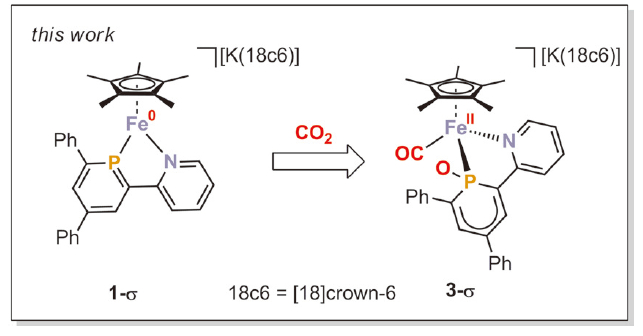
\includegraphics[width=0.55\linewidth]{reax.jpg}\\[0.3cm]
	%	\caption{\footnotesize\fullcite{Leitl}}
	%	\label{fig:reax}
	%\end{figure}
    {\large Shirong Wang}\\[0.3cm]
    Kuang Yaming Honors School\\
    [-0.8cm]}

\date{\today}



\begin{document}
\begin{frame}
Literature Report\hfill ICC Report V
\titlepage
\end{frame}

\begin{frame}
\frametitle{Contents}
\large\tableofcontents
\end{frame}

\section{Background}
%\begin{frame}
%\frametitle{Background}
%Biochemical $ \ce{CO_2} $ reduction
%\begin{columns}
%	\column[]{0.6\linewidth}
%	\begin{figure}
%%		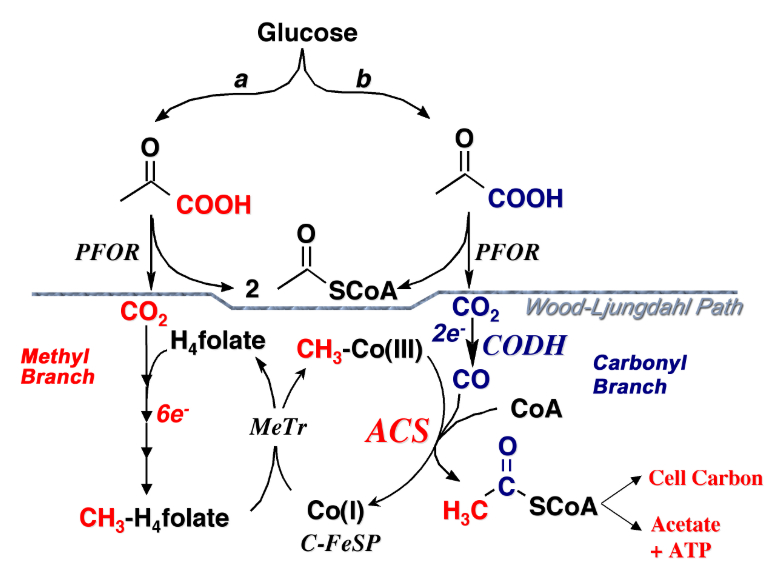
\includegraphics[width=0.7\linewidth]{wood.jpg}
%		\caption{Wood-Ljungdahl Path}
%	\end{figure}
%    \column[]{0.5\linewidth}
%\end{columns}
%
%\end{frame}

\begin{frame}
\frametitle{Background}
$ \ce{C=O} $ Bond Splitting of $ \ce{CO_2} $ has become established
for %highly reducing, 
some d-block metals (Ti, Zr, W, Ir) and f-block metals (U).\\
~\\
However, the use of
earth-abundant 3d metals remains surprisingly under-explored,
particularly given the role that such metals play in
biological $ \ce{CO_2} $ reduction to $ \ce{CO} $, mediated by $ \ce{Ni} $, $ \ce{Fe} $ $ \ce{CO} $ dehydrogenase.
\end{frame}

\begin{frame}
\frametitle{Background}
Previous examples of $ \ce{CO_2} $ cleavage based on 3d metals\\
\begin{figure}
	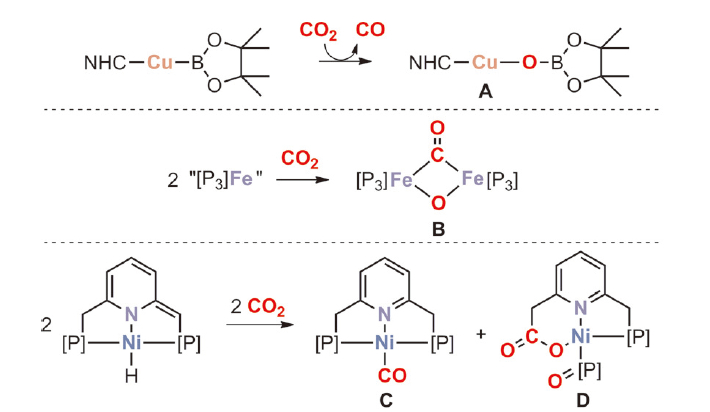
\includegraphics[width=0.7\linewidth]{lit.jpg}
\end{figure}
\hfill\footnotesize\fullcite{laitar2005efficient}\\
\hfill\footnotesize\fullcite{sadique2008reduction}\\
\hfill\footnotesize\fullcite{oren2018metal}
\end{frame}

\begin{frame}
The research of D. Laitar et al. provides a catalytic cycle for $ \ce{CO_2} $ deoxygenation. ICy-cooper catalysis gives 100 turnovers in 1h.
\begin{figure}
	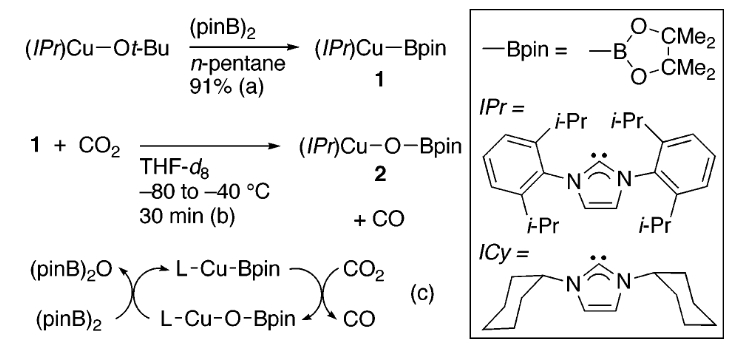
\includegraphics[width=0.7\linewidth]{laitar.jpg}
\end{figure}
\hfill\footnotesize\fullcite{laitar2005efficient}\\
\end{frame}


\begin{frame}
This work is the first reported example of $ \ce{C=O} $ cleavage of a $ \ce{CO_2} $ molecule mediated by a single $ \ce{Fe} $ centre.
\begin{figure}
	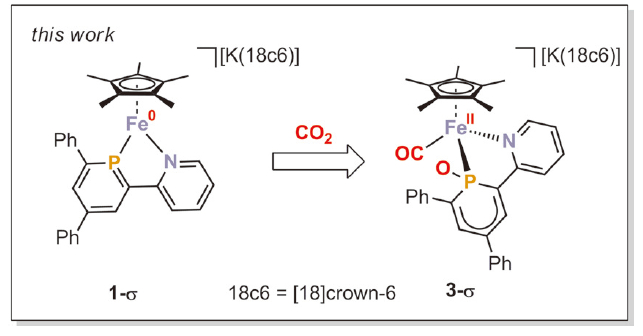
\includegraphics[width=0.6\linewidth]{reax.jpg}
	\caption{\footnotesize\fullcite{Leitl}}
	\label{fig:reax}
\end{figure}
\end{frame}

\begin{frame}
\frametitle{Inspiration}
\begin{columns}
	\column[]{0.7\linewidth}
	\begin{figure}
		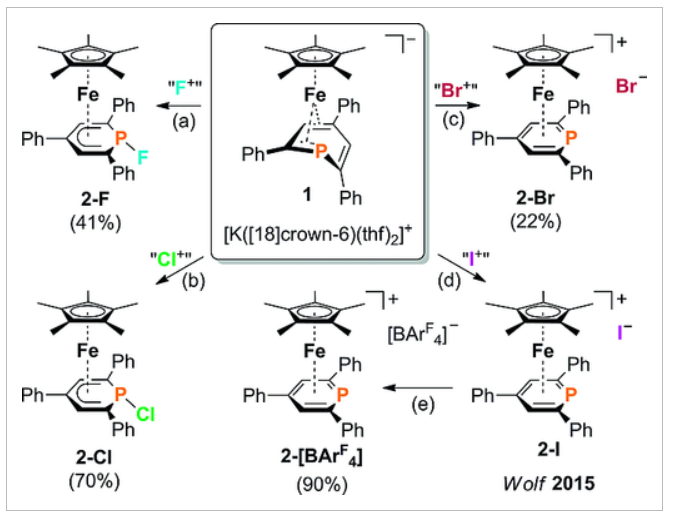
\includegraphics[width=\linewidth]{Fe-TPP.jpg}
		\caption{[Cp*Fe($ \eta^4 $-TPP)] and derived compounds
		\footnotesize\fullcite{Hoidn}}
	\end{figure}
    \column[]{0.3\linewidth}
    \begin{figure}
    	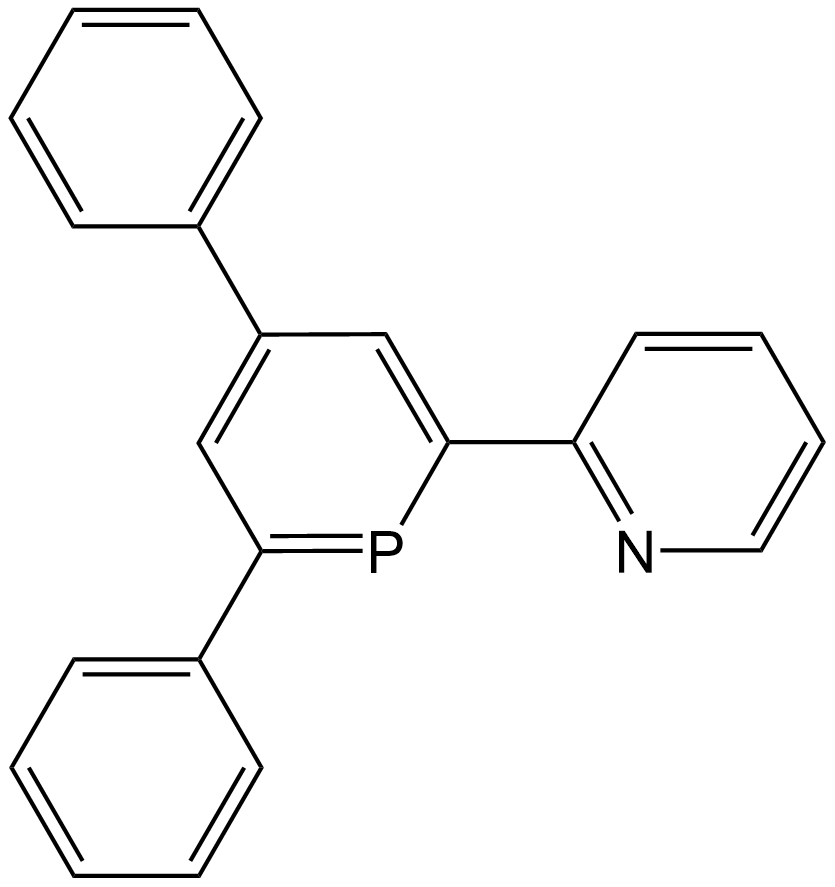
\includegraphics[width=0.7\linewidth]{L.png}
    	\caption{New ligand    2-(2'-pyridyl)-4,6-diphenylphosphinine}
    \end{figure}
\end{columns}

	

%Metal-ligand cooperation
\end{frame}

\section{Reaction Details}
\begin{frame}
\frametitle{Preparation}
\begin{figure}
	\centering
	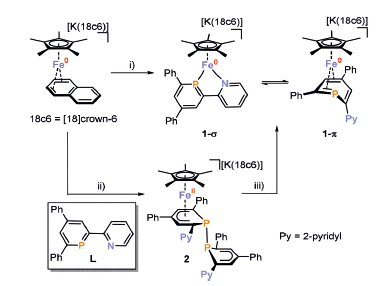
\includegraphics[width=0.65\linewidth]{prep.jpg}
	\caption{i) L, DME, -35\textcelsius to RT, -naphthalene;
		
		     ii) 1 equiv. [K([18]crown-6)][Cp*Fe-(C$ _{10} $H$ _8 $)], 2 equiv. L, toluene/THF, -35\textcelsius to RT; 
		     
		     iii) 1 equiv. [K-([18]crown-6)][Cp*Fe(C$ _{10} $H$ _8 $)], THF.}
\end{figure}
%Solution-phase $ ^{31}P $ NMR spectrum shows 1-$ \sigma $ and 1-$ \pi $, while XRD and $ ^{31}P $ CP MAS show only 1-$ \sigma $.   Selective crystallization failed.\\
%~\\
\end{frame}

\begin{frame}
\frametitle{Calculation for 1-$ \sigma $/1-$ \pi $}
Conversion of 1-$ \pi $ to 1-$ \sigma $ is calculated to proceed with a barrier of \SI{27.0}{kcal/mol}, consistent with an equilibrium at room temperature. NMR indicates an approximately 2:1 ratio of 1-$ \sigma $:1-$ \pi $.
\begin{figure}
	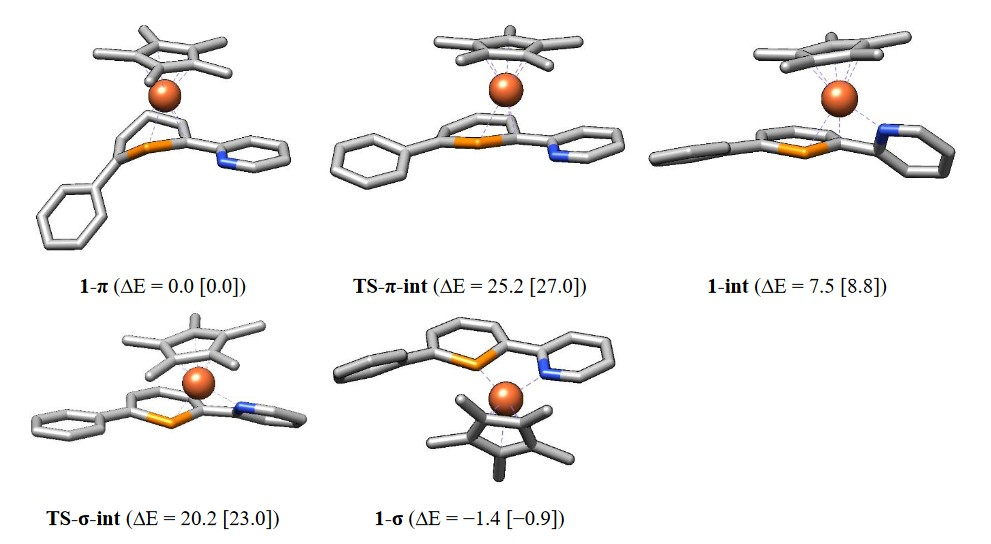
\includegraphics[width=0.8\linewidth]{conver.jpg}
	\caption{Calculation results at TPSSh-D3/def2-TZVP. The geometry is optimized at BP86/def2-TZVP. Both are carried in THF solvent with CPCM model}
\end{figure}
\end{frame}

\begin{frame}
\frametitle{Splitting Reaction}
\begin{figure}
	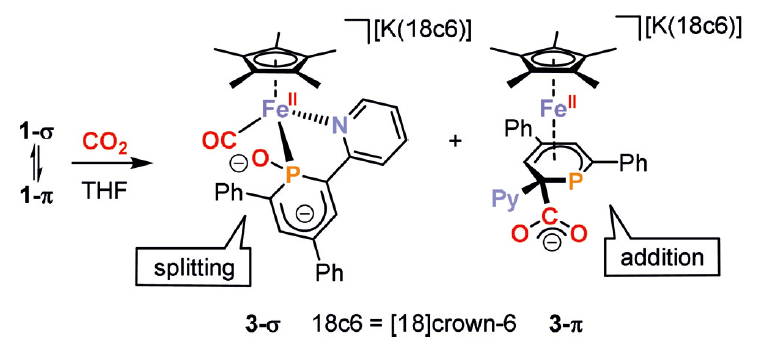
\includegraphics[width=0.7\linewidth]{reax2.jpg}
	\caption{Reaction of 1-$ \sigma $ and 1-$ \pi $ with $ \ce{CO_2} $ (1 atm) in THF at room temperature.}
\end{figure}

\end{frame}

\begin{frame}
Solid state structures of 3-$ \sigma $ and 3-$ \pi $
\begin{figure}
	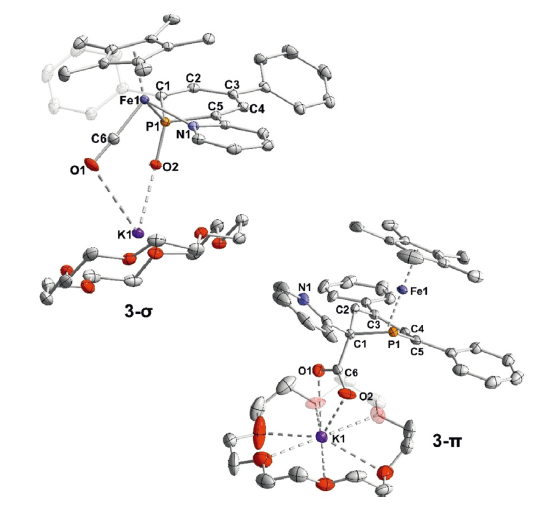
\includegraphics[width=0.7\linewidth]{3.jpg}
\end{figure}

\end{frame}


\begin{frame}
\frametitle{Calculation for 1 $ \rightarrow $ 3 Reaction}
Very small energy barriers:
\begin{itemize}
	\item 1-$ \sigma $ -> 3-$ \sigma $: \SI{3.5}{kcal/mol}
	\item 1-$ \pi $ -> 3-$ \pi $: \SI{5.5}{kcal/mol}
\end{itemize}
\begin{figure}
	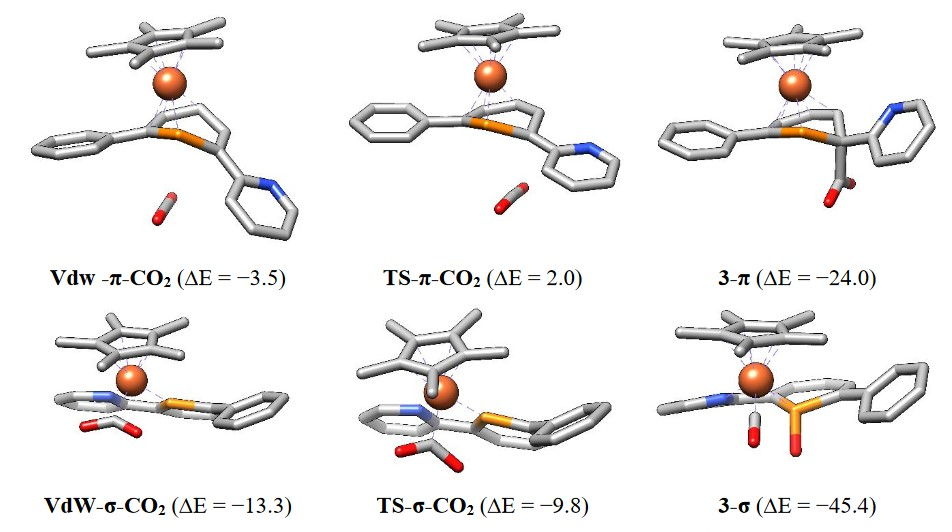
\includegraphics[width=0.85\linewidth]{33.jpg}
	\caption{Calculation results at TPSSh-D3/def2-TZVP. The geometry is optimized at BP86/def2-TZVP. Both are carried in THF solvent with CPCM model}
\end{figure}

\end{frame}



\section{Discussion and Expectations}
\begin{frame}
\frametitle{Discussion and Expectations}
\begin{itemize}
	\item Full catalysation cycle
	\item Diversification of 1-$ \sigma $
	\item Orbital analysis
\end{itemize}

\end{frame}


\section{Current Progress}
\begin{frame}
\frametitle{Current Progress}
Testing calculation with ORCA
\begin{table}
	\centering
	\begin{tabular}{cccc}
		\hline
		method & basis & cores & time\\ \hline
		PBE0-D3 & def2-TZVP/def2-SVP (1758) & 24 & 12h (40 cyc)\\
		PWPB95-D3 & def2-TZVPP (2583) & 72 & 29m\\
		DLPNO-CCSD(T) & def2-TZVPP (2583) & 30 & 18.5h\\
		\hline
	\end{tabular}
\end{table}
Where, RI-J and RIJCOSX used for DFT, RI-MP2 used for Double-hybrid DFT.\\
DLPNO is performed at NormalPNO level. TightPNO calculation is on running for 3 days.
\end{frame}

\end{document}